\documentclass[final]{beamer} 


%=================================================================================
% Document information
\def\firstname{First Name}
\def\familyname{Last Name}
\def\FileAuthor{\firstname~\familyname}
\def\FileTitle{Awesome Title}
\def\FileSubject{File Subject (eg., conference name)}
\def\FileKeyWords{\firstname~\familyname, \FileSubject, \FileTitle}

%=================================================================================
% PACKAGES
\usepackage{amsmath}
\usepackage{amssymb}
\usepackage{amsfonts}
\usepackage{graphicx}
\usepackage[utf8]{inputenc}
\usepackage{textcomp} 
\usepackage{alltt}
\usepackage{subfigure}
\usepackage{latexsym}
\usepackage{eurosym}
\usepackage{verbatim}
\usepackage{epstopdf}         % if you want to use .eps and .jpeg in the same document (compile with pdflatex directly)
\usepackage{array}            % permet d'utiliser m{width} dans l'env tabular
\usepackage{natbib} 
\usepackage[english]{babel}
\usepackage{multirow}

\usepackage{units}
\usepackage{nicefrac}
\usepackage{appendix}
\usepackage{booktabs}
\usepackage{layout}          % then \layout in the document to get the layout numbers
\usepackage{hyperref}         % Hyper references for the document
\hypersetup{
  colorlinks=false,       % false: boxed links; true: colored links
  breaklinks=true,       % permet le retour à la ligne dans les liens trop longs
  linkcolor=black,       % color of internal links (red)
  citecolor=black,       % color of links to bibliography (green)
  filecolor=black,       % color of file links (magenta)
  urlcolor=black,        % color of external links (cyan)
  pdftitle={\FileTitle},
  pdfauthor={\FileAuthor},
  pdfsubject={\FileSubject},
  pdfkeywords={\FileKeyWords}}


% BEAMER specific
\mode<presentation>
\usetheme{default}
\usecolortheme{default} % beetle, lily, beaver

\usepackage{tikz}
\usetikzlibrary{decorations.pathreplacing}
\usetikzlibrary{calc}
\usetikzlibrary{decorations.shapes}
\usetikzlibrary{decorations.pathmorphing}
\tikzset{paint/.style={fill=red}, decorate with/.style={decorate,decoration={shape backgrounds,shape=#1,shape size=3pt}}}
\tikzset{dotr/.style={fill=red!60,circle,minimum size=3pt}}
\tikzset{dotb/.style={fill=blue!60,circle,minimum size=3pt}}
\usetikzlibrary{positioning}
\usetikzlibrary{shapes}

\usepackage{pgfkeys}
\usepackage{multimedia} 
\usepackage{mdwlist}
\usepackage{moreverb}
\usepackage{etex}   % this is a dodgy fix for using lpic: http://www.tex.ac.uk/cgi-bin/texfaq2html?label=noroom
\usepackage{lpic}
\usepackage[absolute,overlay]{textpos} % for absolute positioning on page 

\usepackage[absolute,overlay]{textpos} % for absolute positioning on page
\setbeamertemplate{navigation symbols}{}
\setbeamertemplate{footline}{\leavevmode% 
  \hfill\hbox{% 
    \begin{beamercolorbox}[wd=.15\paperwidth,ht=2.25ex,dp=1ex,right]{date in head/foot}% 
      \scriptsize \insertframenumber{} \hspace*{2ex} 
    \end{beamercolorbox}}% 
  \vskip0pt%
}
\beamertemplatetransparentcovereddynamic
\beamertemplateballitem
\beamertemplatesolidbuttons 

% BEAMERPOSTER specific
\usepackage[size=custom,width=121.92,height=91.44,scale=1,debug]{beamerposter} % from https://groups.google.com/forum/?fromgroups#!topic/beamerposter/O-uDNDwgjyk
\usefonttheme[onlymath]{serif}
\usebackgroundtemplate{\includegraphics[width=\paperwidth,height=\paperheight]{./figs/bkgd}} 
%\usebackgroundtemplate{\includegraphics[width=121.92,height=91.44]{./figs/bkgd}} 
\setbeamertemplate{caption}[numbered]     % number the captions
\setbeamerfont{caption}{size=\normalsize} % make the title of a caption a certain size
\renewcommand{\thesubfigure}{\small (\alph{subfigure})}  % set the subcaption title size
\setbeamertemplate{enumerate item}{\textbf{\insertenumlabel.}} % make the enumerate bullets into plain numbers.
\setbeamertemplate{enumerate subitem}{\insertenumlabel.\insertsubenumlabel}
\setbeamertemplate{enumerate subsubitem}{\insertenumlabel.\insertsubenumlabel.\insertsubsubenumlabel}
\setlength\fboxsep{0pt}
\setbeamerfont{abstract}{size=\small}
\setbeamerfont{abstract title}{parent={abstract,structure},size=\Large,series=\bfseries}


%=================================================================================
% Useful commands
\makeatletter % To get the fontsize: \thefontsize\large
\newcommand\thefontsize[1]{{#1 The current font size is: \f@size pt\par}}
\makeatother
% Needed for the natbib bibliography style
%\newcommand*{\newblock}{}
\bibpunct[<optional>]{}{}{}{s}{}{} 
\def\bibfont{\footnotesize}

%=================================================================================
% Define some colors
\definecolor{violetred}{rgb}{0.78,0.08,0.52}
\definecolor{olivegreen}{rgb}{0.2,0.6,0.0}
\definecolor{darkgray}{rgb}{0.95,0.95,0.95}
\definecolor{mypurple}{rgb}{0.76,0.06,0.76}
\definecolor{greenyellow}{rgb}{0.76,0.76,0.06}
\definecolor{gold}{HTML}{FFD700} 
\definecolor{IMnumber}{HTML}{AFB9DB}

% From http://www.google.com/url?sa=t&rct=j&q=&esrc=s&source=web&cd=1&ved=0CFcQFjAA&url=http%3A%2F%2Fwww.perceptualedge.com%2Farticles%2Fvisual_business_intelligence%2Frules_for_using_color.pdf&ei=TioYUPL8GMPl0QHhqICQAQ&usg=AFQjCNGA9t1pGae49wQ0DVhaSNcAk6oLyA&sig2=QuA9D9nierTbqn3djCyyPQ
\definecolor{c1med}{HTML}{F15A60}
\definecolor{c2med}{HTML}{7AC36A}
\definecolor{c3med}{HTML}{5A9BD4}
\definecolor{c4med}{HTML}{FAA75B}
\definecolor{c5med}{HTML}{9E67AB}
\definecolor{c6med}{HTML}{CE7058}
\definecolor{c7med}{HTML}{D77FB4}
\definecolor{c8med}{HTML}{737373}

\definecolor{c1brt}{HTML}{EE2E2F}
\definecolor{c2brt}{HTML}{008C48}
\definecolor{c3brt}{HTML}{185AA9}
\definecolor{c4brt}{HTML}{F47D23}
\definecolor{c5brt}{HTML}{662C91}
\definecolor{c6brt}{HTML}{A21D21}
\definecolor{c7brt}{HTML}{B43894}
\definecolor{c8brt}{HTML}{010202}

%=================================================================================
% Customize the maketitle command
\defbeamertemplate*{title page}{customized}[1][]
{
  \usebeamerfont{title}\usebeamercolor[white]{title}\veryHuge\inserttitle\par
  \usebeamerfont{subtitle}\usebeamercolor[white]{subtitle}\insertsubtitle\par
  \bigskip
  \usebeamerfont{author}\LARGE\insertauthor\par
  \usebeamerfont{institute}\Large\insertinstitute\par
  \usebeamerfont{date}\insertdate\par
  \usebeamercolor[fg]{titlegraphic}\inserttitlegraphic
}

%=================================================================================
% Title information
\title{Sweet Poster Title}
\author[]{Author McAuthorson $^1$, Dr. Advisorelli $^{1,2}$}
\institute[]{University of Michigan,$^1$Dept. of Epicness, $^2$Dept. of Sammiches }
\date{}


%=================================================================================
% Main document
\begin{document}
  \begin{frame}[plain]{} 
    \begin{center}

      %============================================================================
      % Title stuff
      \begin{textblock*}{30in}[0.5,0.5](0.5\paperwidth,.05\paperheight)
         \maketitle
      \end{textblock*}
      \vspace*{7.5cm}
	
%============================================================================
% First column

      \begin{minipage}[t]{.23\linewidth}
	{\LARGE \structure{\textbf{Section 1's Adventures in Wonderland}}}\\	
	%============
	\begin{block}{\Large Background and Motivation}
	\begin{itemize}
	\item Exciting fact to grab the audience!
	\item Well known, but properly cited fact to add to your credibility. (Fig.\,\ref{fig:FigLabel1}).
	\item A third bullet with some stuff to fill space.
	\end{itemize}
	  \begin{center}
	    \begin{minipage}{1\linewidth}
	  \begin{figure} \def\figurename{Fig.}
	    \centering
	    \includegraphics[width=.9\textwidth,trim = 0cm 3cm 0cm 2cm, clip]{./figs/Chicken}
	    \caption{\normalsize This chicken looks pissed.}
	    \label{fig:FigLabel1}
	  \end{figure}
	    \end{minipage}
	  \end{center}

	\end{block}
	%============
	\begin{block}{\Large Approach}
	\begin{itemize}
	\item Vague generality about what you did.
	\end{itemize}
	  \begin{figure} \def\figurename{Fig.}
	    \centering
	    \includegraphics[width=.9\textwidth,trim = 0cm 7cm 5cm 7cm, clip]{./figs/flower}
	    \caption{\normalsize Here's a picture of a flower because I'm sick of snow.}
	    \label{fig:Problem}
	  \end{figure}
	\end{block}
\begin{itemize}
\item Words...
\item More words...
\item Perhaps  we can put some technical jargon or an impossibly complicated equation here... you know, just to mix things up.
\end{itemize} \vspace*{1cm}
%============
\end{minipage}\hspace{1.25cm}% End of the first column and a good example why you should end your lines with an %
%
%
%
%============================================================================
% Second column
      \begin{minipage}[t]{.23\linewidth}

%============
	{\LARGE \structure{\textbf{Section 2 and the Prisoner of Azkaban}}}\\
	\begin{block}{\Large Subsection Title!}
          \begin{itemize}
	    \item Some facts here
	    \item Some science here.
	    
	  \end{itemize}
  
	  \begin{figure} 
	    \centering
	    \subfigure{{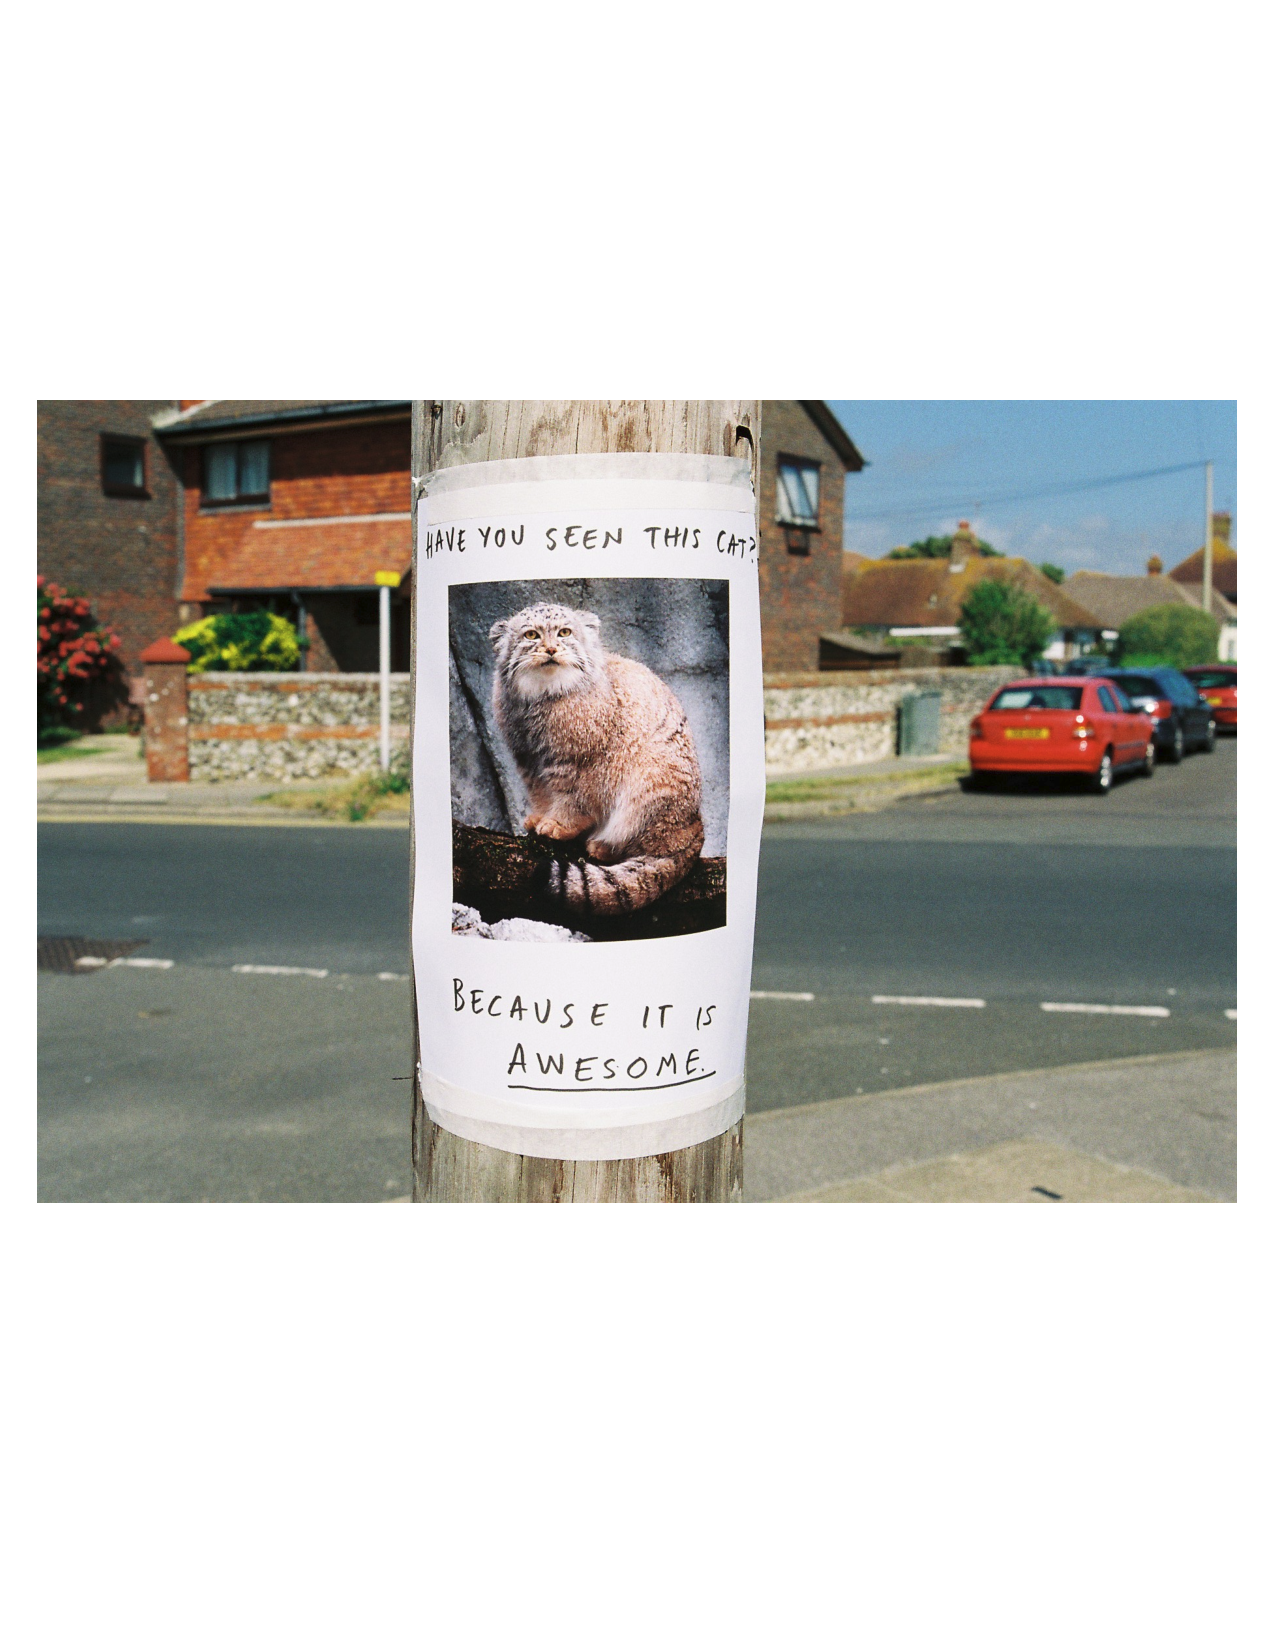
\includegraphics[width=0.45\textwidth,trim = 2cm 7cm 4cm 7cm, clip]{./figs/cat}}}\hspace{.5cm}
	    \subfigure{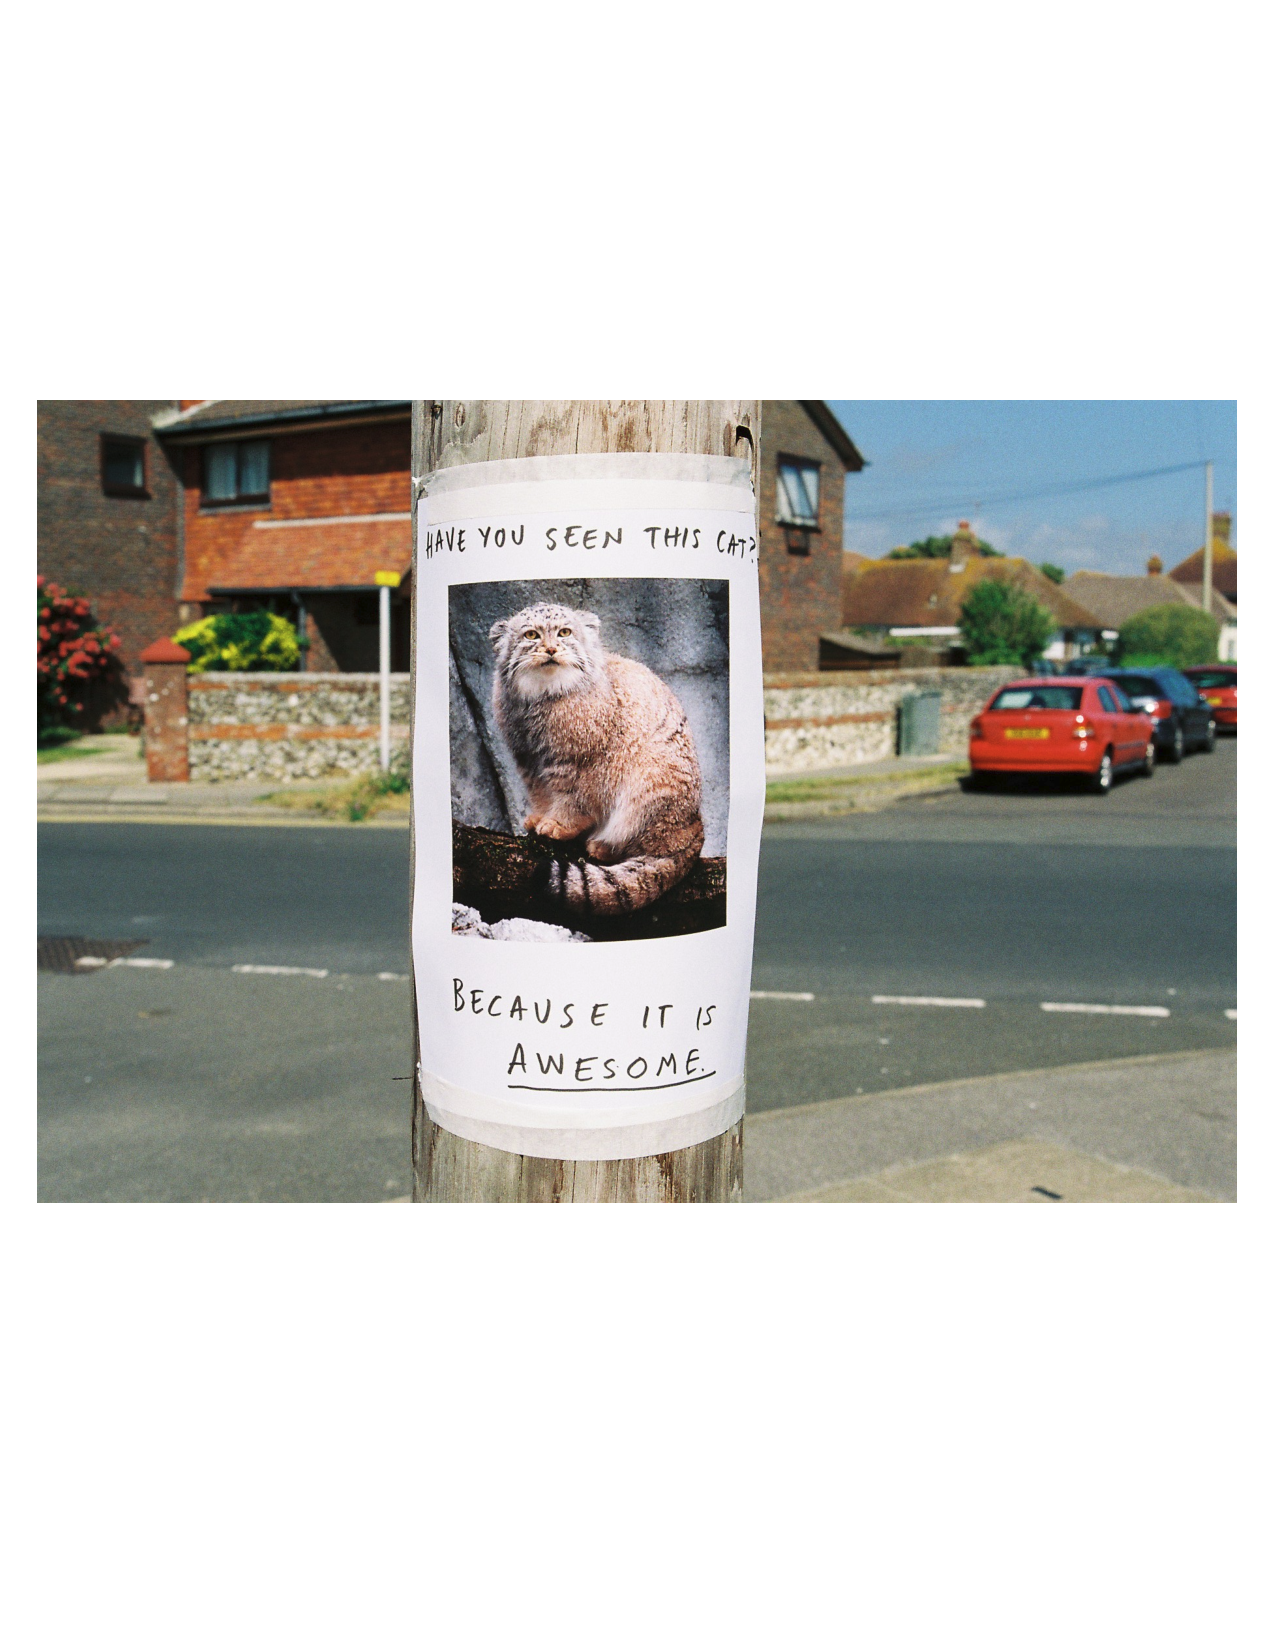
\includegraphics[width=0.45\textwidth,trim = 2cm 7cm 4cm 7cm, clip]{./figs/cat}}\hspace{1cm}
	    \caption{\normalsize These cats are here to teach you the power of subfigures.}
	    \label{fig:CEUS}
	  \end{figure}

	\end{block}\vspace*{1.cm}


        %============
	\begin{block}{\Large Objectives}\vspace*{-0.4cm}
	  \begin{enumerate}\normalsize
	    \item \textbf{Finish this template.}
	    \item \textbf{Make some dinner.}
	    \item \textbf{Get some sleep.}

	  \end{enumerate}
	  
	\end{block} \vspace*{1cm}
	
	        %============
	\begin{block}{\Large Methods}
	  \begin{itemize}
	  \item First, we put the lime in the coconut.
	  \item Then we shook it all up.
	  \item The wall velocity generated cavitation in the coconut, the subsequenuent bubble dynamics were modeled as such,
	  \end{itemize}{\small
	  \begin{align*}
	  \left(1-\frac{\dot{R}}{Ma}\right)R\ddot{R} + \frac{3}{2}\left(1-\frac{\dot{R}}{3 Ma}\right)\dot{R}^2 = \frac{R}{Ma}\left[\left(1+\frac{2}{We}\right)\frac{3\gamma}{R^{3\gamma+1}}\dot{R}+\frac{2\dot{R}}{We R^2} +\dot{\tau}_{rr}\right] \\ \hspace*{-1cm}
	 + \left(1 + \frac{dot{R}}{Ma}\right)\left[\left(1 + \frac{2}{We}\right)\frac{1}{R^{3\gamma}}-\frac{2}{We R} + \tau_{rr} -p_\infty(t) -\frac{R}{Ma}\dot{p}_\infty(t)\right] \hspace*{1cm}
		  \end{align*}}
		  
	\begin{itemize}
	\item Overly complicated numerical schemes were used to solve the above equation because certain members of the faculty don't trust Matlab's ODE45 ) :
	\item The numerical results produced were then stared down until they revealed their secrets.
	\end{itemize}
	
	  \begin{figure} \def\figurename{Fig.}
	    \centering
	    \includegraphics[width=.9\textwidth,trim = 0cm 5cm 0cm 5.5cm, clip]{./figs/seahorse}
	    \caption{\normalsize Things got hard, so the 'sleep-on-it' method (shown above) was employed in order to gain more insight from the results.}
	    \label{fig:FigLabel1}
	  \end{figure}
		  
	\end{block} 

      \end{minipage}\hspace{1.25cm}%
%
%
%
%============================================================================
% Third column
      \begin{minipage}[t]{.23\linewidth}

	{\Large \structure{Results}}\\
	  \begin{figure} \def\figurename{Fig.} 
	    \centering
	    \includegraphics[width=\textwidth, trim=0 40 40 40, clip]{./figs/kangaroo} \vspace*{-2.0cm}
	    \caption{\normalsize An engineering graduate student (right) undergoing of Q \& A from a confused medical doctor (left) after presenting equations.}
	    \label{fig:Bubex}
	  \end{figure}
At this point, I'm adding a disclaimer that these aren't actual scientific results, they're just pics off the internet.
	    \begin{figure} \def\figurename{Fig.}
	    \centering
	    \includegraphics[width=\textwidth, trim=0 150 0 150, clip]{./figs/whoisawesome} \vspace*{-2.0cm}
	    \caption{\normalsize Dog.}
	    \label{fig:Elasticity}
	  \end{figure}
	%%
		\begin{minipage}{\linewidth}
	  \begin{block}{\footnotesize Bibliography}
	    \bibliographystyle{jap}
	    \bibliography{bib}
{\footnotesize	    Note that nothing shows up because I killed my '.bib' file.}
	  \end{block}
	\end{minipage} 
      \end{minipage}\hspace{1.25cm}
%
%
%
%============================================================================
% Fourth column
	\begin{minipage}[t]{.23\linewidth}

		{\Large \structure{Conclusions}}
	\begin{itemize}
	\item Research is hard.
	\item \LaTeX is very useful and looks great, but can suck a bit to get used to.
	\end{itemize}
		\begin{figure} \def\figurename{Fig.}
		\centering
	    \includegraphics[width=\textwidth, trim=60 190 0 190, clip]{./figs/potential} \vspace*{-2.0cm}
		\caption{A visual representation of future job prospects if I keep putting things like this template off until the last minute.}
		\label{fig:PMF}
	      \end{figure}	
	
	\vspace{1.25cm}
			{\Large \structure{Ongoing and Future Work}}
		\begin{figure} \def\figurename{Fig.}
		\centering
	    \includegraphics[width=\textwidth, trim=60 190 0 190, clip]{./figs/n64} \vspace*{-2.0cm}
		\caption{This work is to be conducted over the next 4 years.}
		\label{fig:PMF}
	      \end{figure}

        %============
	\end{minipage}
	
    \end{center}
    
  \end{frame}  
\end{document}



